% *****************************************************************************
%     sections/chapter2.tex
%
% Last edit: 27/03
% *****************************************************************************

\chapter{Bayesian inference of neutron star observables}

% Pulsars were identified to rotating NS which produce pulsed emission (dont
%   know where to put this)

\section{From the equation of state to neutron star observables}

The stellar EoS, the determination of which was studied thoroughly in Chapter 
1, is the fundamental ingredient to build NS models. It enters into the 
basic equation for calculating macroscopic observables relevant to NS, that is 
so-called Tolman-Oppenheimer-Volkoff (TOV) equation, which describes the 
hydrostatic equilibrium for a spherically symmetric star in the framework of 
general relativity~\cite{Tolman1939,Oppenheimer1939}.

This section deals with the estimation of NS observables for several 
popular EoS calculated within the metamodeling technique introduced in 
Chapter 1. In~\ref{subsec:masses}, we first solve the hydrostatic 
equilibrium equations so as to determine the mass-radius relation. The 
thickness and mass of the crust are also evaluated. The calculation of the NS 
moment of inertia in the slow rotation approximation is performed 
in~\ref{subsec:moi}. In particular, we show how the fraction of crust moment 
of inertia is connected to the 
observation of pulsar glitches. In~\ref{subsec:tidal}, we finally compute the 
tidal deformability, which describes how much the NS is deformed by tidal 
forces, arising, for instance, when two NS orbit each other.

\subsection{Masses and radii}\label{subsec:masses}

% observations
From the observational point of view, it is easier for astronomers to measure 
the mass of a NS entering into a binary system. There are several types of
binaries: X-ray binaries, double NS binaries, radio pulsar--white dwarf 
binaries, and radio pulsar--nondegenerate star binaries. Depending on the type 
of binary, different techniques are used to infer the NS 
mass~\cite{Haensel2007}.
% Shapiro delay effect - MSP
For example, in a pulsar binary system, various phenomena, such as the 
relativistic Shapiro delay~\cite{Shapiro1964}, can be measured via pulsar 
timing, which consists of the regular monitoring of the rotation of a a pulsar 
over long periods (years to decades). The relativistic Shapiro delay is a 
phenomenon from which precise masses for both a millisecond pulsar and its 
companion can be inferred~\cite{Demorest2010,Cromartie2020}. Let us notice 
however that it is only observed in a small subset of high-precision, highly 
inclined binary pulsar systems.\\
% Measuring NS radii is less straightforward
Measuring NS radii with high precision is a more challenging task, and it
constitutes one of the goals of the ambitious NICER mission~\cite{NICER}. This
observable can be extracted from the analysis of thermal emission from neutron 
star surfaces, or X-ray emission from accreting neutron stars in binaries.

In the following, we turn to the theoretical prediction of NS masses and radii. 
The hydrostatic equilibrium equations in general relativity are first solved in 
order to represent the mass-radius relation for several popular EoS, which are
then confronted to NS mass measurements. The estimation of the crustal 
thickness and mass is discussed afterwards.

\subsubsection{Mass-radius relation}

% hydrostatic equilibrium in GR
Theoretically, the NS masses and radii correspond to the 
solution of the hydrostatic equilibrium equations, which are, in general 
relativity for spherical and nonrotating 
stars~\cite{Tolman1939,Oppenheimer1939},
%
\begin{eqnarray}
  \frac{dP}{dr} &=& -\frac{G\rho_B m}{r^2}\left(1 + \frac{P}{\rho_B
  c^2}\right)\left(1+\frac{4\pi
  Pr^3}{mc^2}\right)\left(1-\frac{2Gm}{rc^2}\right)^{-1},\label{eq:tov}\\
      \frac{dm}{dr} &=& 4\pi r^2\rho_B,\label{eq:massbal}\\
  \frac{d\Phi}{dr} &=& -\frac{1}{\rho_B
    c^2}\frac{dP}{dr}\left(1+\frac{P}{\rho_B
  c^2}\right)^{-1}\label{eq:metric},
\end{eqnarray}
%
where $G$ is the gravitational constant, $P$ the pressure, $\rho_B c^2$ the
energy density, and $m(r)$ the is the gravitational mass inside the sphere of
radius $r$, defined within the Schwarzschild metric $ds^2 = c^2dt^2e^{2\Phi} 
- e^{2\lambda}dr^2 - r^2(d\theta^2 + \sin^2\theta d\phi^2)$. The function 
$\Phi(r)$ corresponds to the gravitational potential, and $\lambda(r)$ is 
related to the enclosed mass $m(r)$ through
%
\begin{equation}
  e^{-\lambda} = \sqrt{1-\frac{2Gm}{rc^2}}.
\end{equation}
%
% description of the equations
Eq.~(\ref{eq:tov}) is the TOV equation 
of hydrostatic equilibrium. The integration of Eq.~(\ref{eq:massbal}) from
$r=0$ to the boundary $r=R$, $R$ being the NS radius, gives the total
gravitational mass $M=m(R)$ of the star. Eq.~(\ref{eq:metric}) is a 
relativistic equation for the metric function $\Phi(r)$. Here, we focus on 
solving Eqs.~(\ref{eq:tov}) and 
(\ref{eq:massbal}), which gives the profiles $P(r)$, $\rho_B(r)$, and $m(r)$ 
for a given EoS, $P(\rho_B)$, the determination of which was discussed in 
detail in Chapter 1.

% explain numerical method for a central density nc (CGS, Euler method, 
%   lagrangian interpolation)
In view of solving the hydrostratic equilibrium equations for a given tabulated 
EoS, one first have to choose an arbitrary value for the central density 
$\rho_{B,c}$ and 
interpolate the central pressure $P_c = P(\rho_{B,c})$, corresponding to $r=0$, 
with the associated boundary condition $m(r=0) = 0$. Then, using a Runge-Kutta 
method, one integrate up to $r=R$, defined as $P(r=R) = 0$ (our numerical 
condition is $P < 5\times 10^{-4}$ MeV/fm$^{3}$, which is a sufficiently low 
value of the pressure). At each new step of pressure, one has to interpolate 
the mass density $\rho_B$ in the table. In the end, for a given value of 
central density $\rho_{B,c}$, one obtains the profiles $P(r)$, $\rho_B(r)$, 
and $m(r)$, and therefore a value for the NS mass $M$ and radius $R$. The 
typical values of these observables are $M=1.4M_\odot$ and $R=10$ 
km~\cite{Haensel2007}.\\
% The problem is that the central density inside a NS is not known... thats why 
%   we are interested in the Mass radius relation
In fact, the central density inside a specific NS is not known, and is expected
to range from $\approx 4.6\times 10^{14}$ g/cm$^3$ to $\approx 4\times 10^{15}$
g/cm$^3$. For this reason, we are rather interested in the mass-radius 
relation, which can be obtained by calculating $M$ and $R$, following the 
numerical method previously explained, for this range of central mass 
densities.\\
% efld
Let us recall that one has to redefine the high-order parameters $Q_{sat(sym)}$ 
and $Z_{sat(sym)}$ in order to reproduce existing functionals at densities
greater than $2n_{sat}$ with the metamodeling technique. This corresponds to
the ELFd technique introduced in \cite{Margueron2018a}.

\begin{table}[!t]
\begin{center}
\begin{tabular}{cccccc} 
  \toprule
  \toprule
  Parameter & Unit & $N$ & BSk14 & PKDD & TM1\\
  \midrule
  $E_{sat}$ & MeV & 0         & -15.85 & -16.27  & -16.26 \\
  $n_{sat}$ & fm$^{-3}$ & 1   & 0.1586 &  0.1495 & 0.1450 \\ 
  $K_{sat}$ & MeV & 2         & 239    &  261    & 281    \\ 
  $Q_{sat}$ & MeV & 3         & -359   &  -119   & -285   \\ 
  $Z_{sat}$ & MeV & 4         & 1435   &  4213   & 2014   \\ 
  $E_{sym}$ & MeV & 0         & 30.00  &  31.19  & 36.94  \\
  $L_{sym}$ & MeV & 1         & 43.9   &  79.5   & 111.0  \\
  $K_{sym}$ & MeV & 2         & -152   &  -50    & 34     \\
  $Q_{sym}$ & MeV & 3         & 389    &  -28    & -67    \\
  $Z_{sym}$ & MeV & 4         & -2191  &  -1315  & -1546  \\
  $m_{sat}^*/m$ & &           & 0.80   &  0.65   & 0.71   \\
  $\Delta m_{sat}^*/m$ & &    & 0.03   &  -0.08  & -0.09  \\
  \bottomrule
  \bottomrule
\end{tabular}
\end{center}
\caption[Empirical parameters for BSk14, PKDD, and TM1]{Value of each of the 
  empirical parameters ,associated unit, and derivative order $N$ for BSk14 
  \cite{Goriely2007}, PKDD \cite{Long2004}, and TM1~\cite{Sumiyoshi1995} 
functionals.}\label{table:newemppar}
\end{table}

\begin{figure}[!t]
\begin{center}
  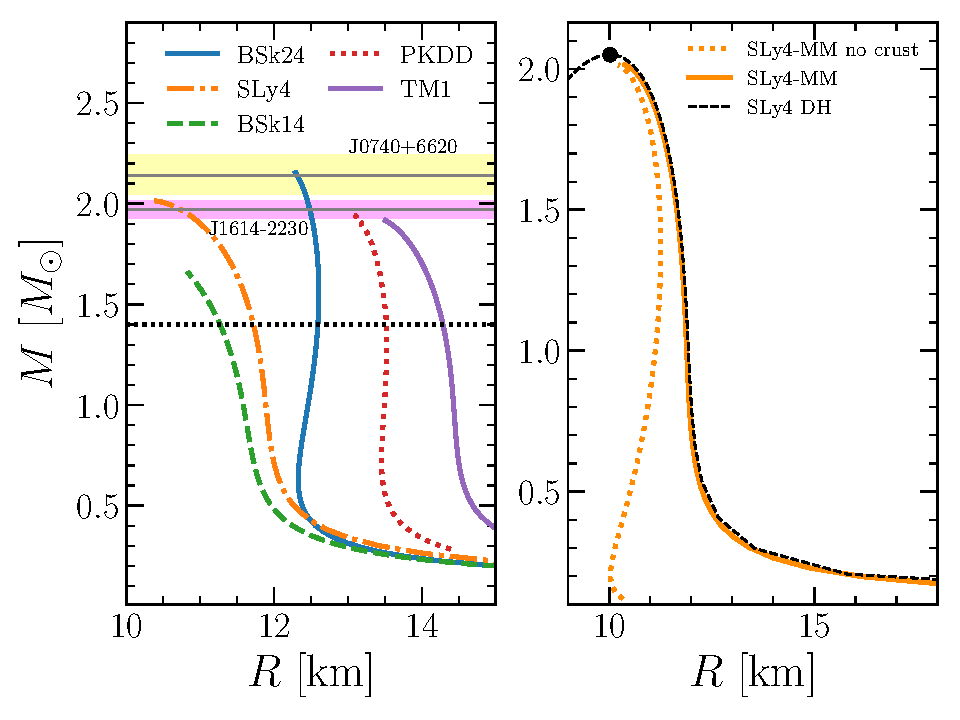
\includegraphics[width=0.9\linewidth]{figures/mr_popular.pdf}
\end{center}
\caption[Mass-radius relation for several popular equations of state]{Left: 
  Mass-radius relation for several popular EoS calculated
  with the metamodeling technique. The black dotted line marks the NS 
canonical mass, that is $1.4M_\odot$. The magenta band represents the measured 
mass of PSR J0348+0432, $(2.01 \pm 0.04)M_\odot$ \cite{Antoniadis2013}, and the 
yellow band that of PSR J0740+6620, $2.14_{-0.09}^{+0.10}M_\odot$ ($68.3\%$ 
credibility interval) \cite{Cromartie2020}.
Right: Mass-radius relation for the DH EoS for SLy4 functional (black dashed
line), and the SLy4 EoS calculated with the metamodeling technique (solid
orange line). The black circle indicates the maximum 
mass.}\label{fig:mr_popular}
\end{figure}
 
The left panel of Fig.~\ref{fig:mr_popular} shows the mass-radius relation for 
several popular EoS based on Skyrme-type functionals BSk24, SLy4, and BSk14, 
and relativistic models PKDD and TM1, calculated within the metamodeling 
technique. A strong model dependence is observed, with radii of canonical NS 
ranging from $R_{1.4}=11.5$ km for BSk14 to $R_{1.4}=14.5$ km for TM1. More
specifically, it is seen that the radius is positively correlated to the slope 
of the symmetry energy $L_{sym}$. The value of the empirical parameters 
associated to BSk14, TM1, and PKDD are reported in Table~\ref{table:newemppar}, 
whereas those of BSk24 and SLy4 can be found in Table~\ref{table:emp_params}.\\
The bands correspond to the measured masses of the two most massive
pulsars observed to the present day. The mass of PSR J0348+0432 was precisely 
estimated to $(2.01\pm 0.04)M_\odot$~\cite{Antoniadis2013}, and the very recent
relativistic Shapiro delay measurements of PSR J0740+6620 led to 
$2.14_{-0.09}^{0.10}M_\odot$ ($68.3\%$ credibility
interval)~\cite{Cromartie2020}. Naturally, if an
EoS cannot insure such high masses, it should not be considered as reliable, 
in particular at high density, since the maximum mass is determined by the 
stellar core EoS. In particular, it is seen that the maximum mass corresponding
to the BSk14 functional, $1.8M_\odot$, is lower than the measured mass
of PSR J0348+0432. Also, while the SLy4 EoS satisty this constraint, the maximum 
mass for this EoS, $2.05M_\odot$, is lower than that of PSR J0740+6620. This 
outline the fact that measuring the mass of pulsars is important, because it 
provides a strong constraint on the stellar matter EoS. Similarly, the NICER
telescope is expected to provide, for years to come, a constraint on the NS
radii with a precision of $5\%$. Ultimately, in the ideal case where one could 
accurately measure the mass and radius of one neutron star, it would be 
possible to determine the EoS by positioning the point in the $M-R$ diagram.

The mass-radius relation for the SLy4 EoS is represented in the right panel of
Fig.~\ref{fig:mr_popular}. The solid orange line corresponds to $M(R)$ for the 
SLy4 EoS calculated within the metamodeling technique, and the dashed 
black line is the calculation based on the DH EoS for SLy4 functional. A 
perfect agreement is observed between the two curves, reflecting the small 
error on the EoS, illustrated in Fig.~\ref{fig:unified}. \\
The dotted orange line shows the mass-radius relation for the SLy4 EoS without
considering the clustering of matter at low density, that is assuming that the
NS star interior consists of $npe\mu$ matter at all densities. In that case,
for a canonical NS, we find $R_{1.4} = 11.1$ km, which is almost $1$ km lower 
with respect to the result with a crust EoS. Moreover, this difference is found 
to be larger with decreasing mass. This shows that the crust EoS is essential 
to properly predict NS radii. However, we can see that the NS maximum mass is 
entirely determined by the stellar core EoS.\\
The black point marks the maximum mass for the SLy4 EoS, $M_{max} = 
2.05M_\odot$. Let us notice that the branch left to the point is unstable, 
because from this point the mass decreases with central density increasing.

\subsubsection{Crust thickness and mass}
% crust thickness and mass
As explained in Chapter 1, a precise estimation of the CC transition point is
required as far as crustal properties are concerned. In particular, the
transition pressure $P_t$ is essential for the determination of the thickness 
and mass of the crust, given respectively by $l_{crust}=R-R_{core}$ and
$M_{crust}=M-M_{core}$, with $R_{core}$ ($M_{core}$) the radius
(mass) of the stellar core. Indeed, in order to caclulate the core radius and
mass, which are involved in the calculation of the crustal observables, one has 
to integrate the hydrostatic equilibrium equations, Eqs.~(\ref{eq:tov}) and 
(\ref{eq:massbal}), from $r=0$ to $r=R_{core}$, defined as $P(r=R_{core})=P_t$.

\begin{figure}[!t]
\begin{center}
  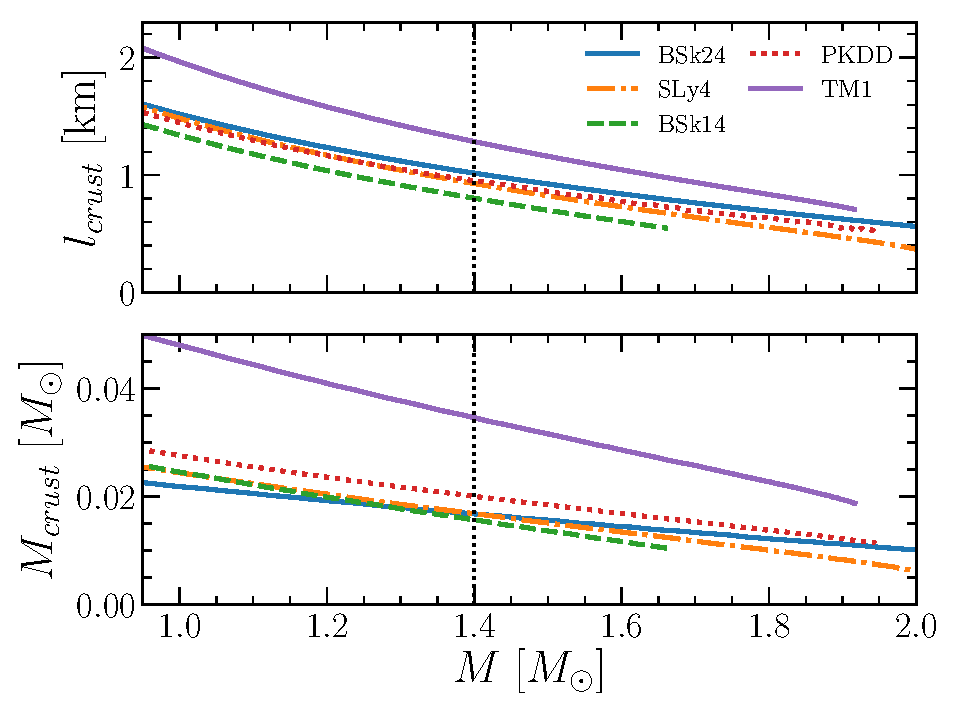
\includegraphics[width=0.9\linewidth]{figures/crustmassthick.pdf}
\end{center}
\caption[Crust thickness and mass versus neutron star mass for several 
popular equations of state]{Crust 
  thickness $l_{crust}$ (upper panel) and mass $M_{crust}$ (lower panel) as a 
  function of the NS mass $M$ for several popular EoS calculated within the 
  metamodeling technique. The black dotted line marks the NS canonical mass, 
  that is $1.4M_\odot$.}\label{fig:crustmassthick}
\end{figure}

Fig.~\ref{fig:crustmassthick} shows the variation with NS mass of crust 
thickness $l_{crust}$ and mass $M_{crust}$ for the same EoS as in 
Fig.~\ref{fig:mr_popular}. As previously, the high-order empirical parameters
are reevaluated to calculate the EoS entering into the TOV equation. However,
the transition pressure is calculated using the values of $Q_{sat(sym)}$ and
$Z_{sat(sym)}$ directly derived from the selected functionals. The reason is
that, as showed in Fig.~\ref{fig:sly4_nt}, the determination of CC transition 
point is sensitive to orders $N>2$.\\
We find the interesting result that the crust is thicker for low-mass neutron 
stars, and in consequence that the $M_{crust}$ drops continuously with 
increasing NS mass. At $M=1.4M_\odot$ (black dotted line), we 
observe that the crust is $\approx 1$ km thick, and that the crust mass is 
approximately $0.02-0.04M_\odot$, which is $(1.5-3)\%$ of the total mass. Once
again, a model dependence is observed. Nonetheless, the correlation of the 
crust thickness with the slope of the symmetry energy is 
not clear. In Fig.~\ref{fig:mr_popular}, we have seen that the radius of the 
star is positively correlated with $L_{sym}$. In fact, the same is true for the 
core radius, explaining why the correlations cancel in the crust 
thickness $l_{crust} = R - R_{core}$.

\subsection{Moment of inertia within the slow rotation
approximation}\label{subsec:moi}

We now turn to the calculation of the moment of inertia within the slow 
rotation approximation~\cite{Hartle1967}. In 
fact, this approximation is not only applicable to slowly rotating pulsars but 
is also reliable for most of them. Indeed, while many observed pulsars show  
rapid rotation~\cite{Stovall2013}, their structure is almost not altered by it 
since centrifugal forces are small in comparison to the gravity, 
$R^3\Omega^2/(GM) \ll 1$, $\Omega$ being the angular frequency. For instance, 
let us consider a rapidly rotating pulsar with $\Omega = 1000$ s$^{-1}$ and 
canonical values for its mass and radius, $M=1.4M_\odot$ and $R=10$ km. In that 
case, we find $R^3\Omega^2/(GM) \approx 0.025$.

In the following, we first calculate the total moment of inertia and the 
fraction of it contained in the NS crust for several popular EoS. Then, we 
explain the connection between the fraction of crust moment of inertia 
and the glitch behavior exhibited by some pulsars~\cite{Espinoza2011}.

\subsubsection{Total moment of inertia and fraction contained in the crust}

In a slowly rotating NS, the total moment of inertia is given
by~\cite{Hartle1967}
%
\begin{equation}
  I = \frac{8\pi}{3}\int_0^R dr r^4\left(\rho_B +
  \frac{P}{c^2}\right)
  \frac{\bar{\omega}}{\Omega}e^{-\lambda-\Phi}\label{eq:moi},
\end{equation}
%
where we have introduced the rotational drag function $\bar{\omega}(r)$, which
satisfies
%
\begin{equation}
  \frac{d}{dr}\left(r^4j\frac{d\bar{\omega}}{dr}\right) =
  -4r^3\bar{\omega}\frac{dj}{dr},\label{eq:rotdrag}
\end{equation}
%
with $j=e^{-\Phi-\lambda}$. Eq.~(\ref{eq:rotdrag}) satisfy the following
boundary conditions at the surface and center of the NS, respectively:
%
\begin{equation}
  \frac{1}{\Omega}\bar{\omega}(r=R) = 1 - \frac{2GI}{R^3c^2} \quad \text{and} 
  \quad \frac{d\bar{\omega}}{dr}\bigg|_{r=0} = 0.
\end{equation}
%
One can translate Eq.~(\ref{eq:rotdrag}) into a first-order differential
equation by introducting $w = (1/\Omega)d\ln\bar{\omega}/d\ln r$, yielding
%
\begin{equation}
  \frac{dw}{dr} = \frac{4\pi G}{c^2}\frac{(P+\rho_Bc^2)(4+w)r^2}{rc^2-2Gm} -
  \frac{w}{r}(3+w)\label{eq:rotdrag2},
\end{equation}
%
with the boundary condition $w(r=0) = 0$. This equation is solved together with 
Eqs.~(\ref{eq:tov}) and (\ref{eq:massbal}) in order to calculate the total 
moment of inertia, which can be rewritten as
%
\begin{equation}
  I = \frac{c^2}{G}\frac{w(R)R^3}{6 + 2w(R)}.
\end{equation}
%
The fraction of crust moment of inertia can also be calculated 
as~\cite{Lim2019}
%
\begin{eqnarray}
  \frac{I_{crust}}{I} &=& 1 - \frac{I_{core}}{I}\notag\\
                      &=& 1 - \left(\frac{R_{core}}{R}\right)^3
                      \frac{w(R_{core})}{w(R)}
                      \exp\left[-\int_{R_{core}}^{R}\frac{w(r)}{r}dr\right],
\end{eqnarray}
%
where we have introduced the moment of inertia of the core $I_{core}$, defined
by the integration of Eq.~(\ref{eq:moi}) up to the core radius $R=R_{core}$.

\begin{figure}[!t]
\begin{center}
  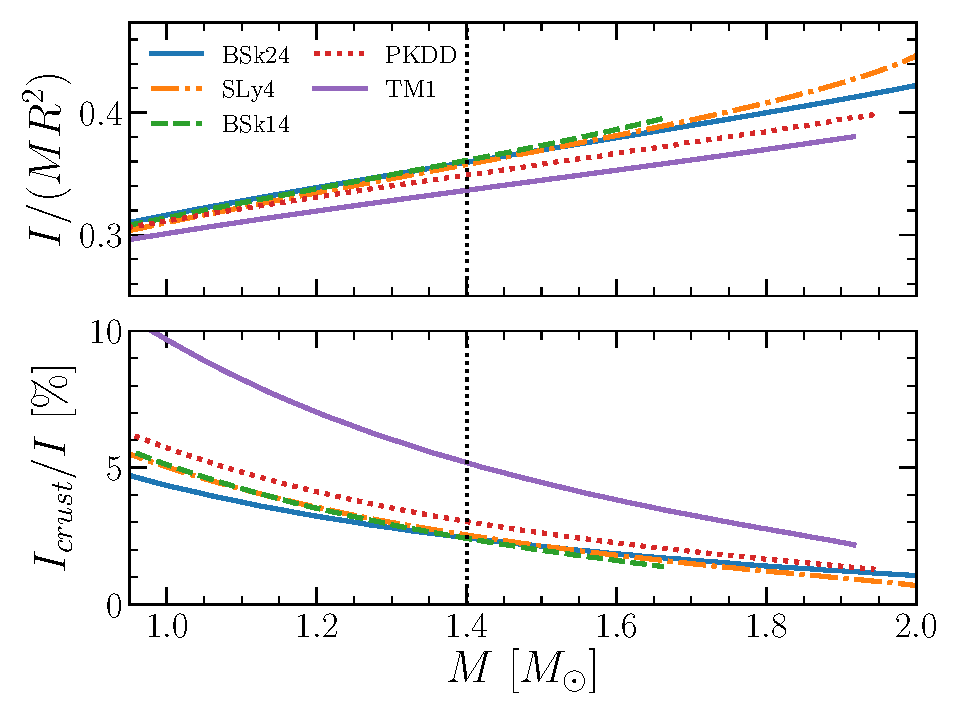
\includegraphics[width=0.9\linewidth]{figures/moi_popular.pdf}
\end{center}
\caption[Moment of inertia and fraction of crust moment of inertia
versus neutron star mass for several popular equations of state]{Moment of
  inertia $I$ (upper panel) and fraction of crust moment of inertia
  $I_{crust}/I$ (lower panel) as a function of the NS mass $M$ for several 
  popular EoS calculated within the metamodeling technique. In the upper panel, 
  the black dotted line marks the NS canonical mass, that is $1.4M_\odot$. In
the lower panel, the minimum values needed to justify Vela glitches with
(Delsate \textit{et al.}~\cite{Delsate2016} and Andersson \textit{et
al.}~\cite{Andersson2012}) and without (Link \textit{et al.}~\cite{Link1999}) 
crustal entrainment are represented.}\label{fig:moi_popular}
\end{figure}

The total moment of inertia is plotted as a function of the NS mass in the
upper panel of Fig.~\ref{fig:moi_popular} for EoS based on Skyrme-type
functionals BSk24, SLy4, and BSk14, and relativistic models PKDD and TM1.
For $M=1.4M_\odot$, it is found that $I$ ranges from $\approx 1.2\times 
10^{45}$ g cm$^2$ for the soft BSk14 EoS to $\approx 2\times 10^{45}$ g cm$^2$ 
for the very stiff TM1 EoS. This shows the strong dependence on the EoS. More 
particularly, an apparent positive correlation with $L_{sym}$ is observed. 
It is seen that the model dependence is even larger for high-mass NS.

The lower panel of Fig.~\ref{fig:moi_popular} shows the variation with NS mass
of $I_{crust}/I$ for the same EoS. It is seen that the more massive a 
NS is, the less moment of inertia it stores in its crust, which follows
the trends observed in Fig.~\ref{fig:crustmassthick}. This was predictable from 
the sensitivity of crustal properties to the CC transition pressure. Given the 
selected EoS, the value of $I_{crust}/I$ at $M=1.4M_\odot$ 
ranges from $\approx 2\%$ for BSk14 to $\approx 5\%$ for TM1, showing once 
again the dramatic dependence on the EoS.

\subsubsection{Connection to pulsar glitches}\label{subsubsec:glitch}

The so-called pulsar glitches are sudden jumps in the rotational frequency of 
a compact star. They are thought to originate from an abrupt transfer of 
angular momentum from the liquid interior, acting as an angular momentun
reservoir, to the solid crust of the star due to the unpinning of the 
superfluid vortices from the crystal lattice~\cite{Anderson1975}. This occurs 
when the differential lag between the slower solid crust and faster superfluid 
vortices reach some threshold and can no longer be sustained, so as to recover 
a close equilibirum between the two. Eventually, stresses start to build up 
again, ultimately leading to another glitch event.

At the time of writing, 555 glitches have been observed in 190 pulsars through 
high-precision pulsar timing~\cite{Espinoza2011,Glitches}. For a given 
glitcher, three quantities are usually measured: its spin frequency $\Omega$, 
its average spin-down rate $\dot{\Omega}$, and its glitch activity parameter
$\mathcal{A}$, defined as
%
\begin{equation}
  \mathcal{A} = \frac{1}{t}\sum_{i=1}^{N} \frac{\Delta \Omega_i}{\Omega},
\end{equation}
%
where $\sum_i \Delta\Omega_i/\Omega$ represents the cumulative spin-up rate
over the $N$ glitches occuring during a time $t$.

It was demonstrated in~\cite{Link1999} that the ratio of the moment of inertia
associated to the neutron superfluid which drives the glitches $I_{sf}$ to the 
moment of inertia of the solid crust -- plus any portion of the star strongly 
coupled to it -- $I_c$ must satisfy 
%
\begin{equation}
  \frac{I_{sf}}{I_c} \geq \frac{\Omega}{|\dot{\Omega}|}\mathcal{A} 
  \equiv \mathcal{G},
\end{equation}
%
where we have introduced the coupling parameter $\mathcal{G}$. In view of
relating the observational constraint $\mathcal{G}$ to the fractional moment of
inertia $I_{crust}/I$ to ultimately set a constraint on the stellar EoS, we 
assume that the angular momentum reservoir is confined to the neutron 
superfluid coexisting with the crystal lattice of the inner crust. In that 
case, we have $I_c = I - I_{res} \simeq I$ and $I_{crust} \simeq I_{sf}$,
yielding~\cite{Link1999}
%
\begin{equation}
  \frac{I_{sf}}{I_c} \simeq \frac{I_{crust}}{I} 
  \geq \mathcal{G}\label{eq:noent}.
\end{equation}
%

In reality, the neutron superfluid is strongly coupled to the solid crust due
to nondissipative entrainment effects~\cite{Chamel2013}, limiting the amount of
angular momentum that can be transfered during a glitch event. The importance
of the entrainment coupling is related to the neutron effective mass $m_n^*$ in
the inner crust, which is proportional to the ratio of unbound neutrons to 
those that are not entrained, $m_n^* \equiv m_n n_g/n_g^c$. Taking into 
account the entrainment effects, the previous constraint, Eq.~(\ref{eq:noent}), 
then becomes~\cite{Andersson2012}
%
\begin{equation}
  \frac{I_{crust}}{I} \geq \mathcal{G}\frac{\langle m_n^* \rangle}{m_n},
\end{equation}
%
with $\langle m_n^* \rangle$ the average effective neutron mass.
It should be stressed that systematic calculations of $m_n^*$ throughout 
the NS crust are very costly from the computational point of view and that,
following~\cite{Andersson2012,Piekarewicz2014}, we adopt the 
value $\langle m_n^* \rangle /m_n = 4.3$, which is inferred from the 
results of~\cite{Chamel2012}. Naturally, one recover the expression without 
crustal entrainment in the case of $\langle m_n^* \rangle = m_n$. We should 
stress that the importance of the effect of crustal entrainment, that is the 
value of the average neutron effective mass throughout the solid crust, is 
currently under debate~\cite{Martin2016,Watanabe2017}.

The Vela pulsar (B083345-45) is one of the most active glitchers known, with
glitches occuring four times per decade on average. Since the beginning of its 
monitoring, almost than 50 years ago, it has exhibited 20 glitches in
total~\cite{Glitches}, allowing for a precise estimation of the corresponding 
the coupling parameter, $\mathcal{G}_{Vela} = (1.62 \pm 0.03) \times
10^{-2}$~\cite{Ho2015}. This can be translated into a constraint for 
the fraction of crust moment of inertia,
%
\begin{equation}
  \left(\frac{I_{crust}}{I}\right)_{Vela} \geq (1.62 \pm 0.03) \times 10^{-2}
  \frac{\langle m_n^* \rangle}{m_n} \approx 0.07.
\end{equation}
%
In other words, in the standard picture where the angular momentum reservoir is 
exclusively confined to the neutron superfluid permeating the inner crust, the 
crust must store more than $7\%$ (with entrainment effects included) of the 
total moment of inertia in order to justify the large glitches occuring in the 
Vela pulsar.

The Vela constraints on $I_{crust}/I$ are displayed in the lower panel of 
Fig.~\ref{fig:moi_popular}. Neglecting entrainment effects~\cite{Link1999}, it
is seen that the constraint is easily satisfied. For BSk14 EoS, which is the
softest EoS here, it leads to $\approx 1.6M_\odot$ for the maximum mass of 
Vela. Now including crustal entrainment with $\langle m_n^*\rangle/m_n =
4.3$~\cite{Andersson2012}, it is not clear, due to dependence on the EoS, 
whether the superfluid neutron in the crust can carry enough angular momentum 
to explain Vela glitches. For the three nonrelativistic Skyrme-based EoS that 
we consider, we see that the constraint is unlikely to be satisfied, because it
would require the Vela mass to be very low, $M_{Vela} \lesssim 0.9M_\odot$.
While theoretically plausible~\cite{Haensel2007}, such low-mass NS have never 
been observed to this day. On the other hand, it is observed that very stiff 
EoS such as TM1 can be consistent with the constraint~\cite{Piekarewicz2014}.
Finally, given the constraint on the fractional moment of inertia calculated 
with the present largest estimation of crustal entrainement~\cite{Delsate2016}
(black thick line), we find that the inferred mass of Vela is at most 
$\approx 0.85M_\odot$ for the stiff TM1 EoS and $\approx 0.65M_\odot$ for the 
soft EoS based on Skyrme functionals. Clearly the question 
``\textit{Is the crust enough?}'' deserves further investigations. In that 
sense, it will be addressed in~\ref{subsec:gli_stats} in the context of a 
complete statistical analysis~\cite{Carreau2019moi}.

\subsection{Tidal deformability}\label{subsec:tidal} % 2

The tidal deformability describes how much a body is deformed by tidal forces,
which arise when two massive bodies orbit each other. The simplest example
corresponds of course to the Moon causing the tides observed in Earth's 
oceans.
The detection of gravitational radiation emitted by inspiraling binary NS 
is possible using ground-based gravitational wave (GW) detectors such as LIGO 
and Virgo. 
Shortly before merging, once the relative distance between the stars is small
enough, the tidal distortion of the NS becomes so large that, in some cases (in
strongest signals), it becomes possible to infer the tidal deformability from 
the GW signal. Theoretically, the tidal deformability parameter is the 
observable which makes the link between the EoS and the gravitational signal. 
In that sense, GW observations can ultimately provide new constraints on the 
EoS. In particular, the first dectection of GW from the coalescence of two NS, 
the GW170817 event, have yielded a value for the tidal deformability of a 
$1.4M_\odot$ NS~\cite{GW1}.

Let us consider a static, spherically symmetric NS, placed in a static external
quadrupolar tidal field $\mathcal{E}_{tid}$. The induced quadrupole moment of
this star is given by 
%
\begin{equation}
  Q_{tid} = -\lambda \mathcal{E}_{tid},
\end{equation}
%
where $\lambda$ is the tidal deformability, which is related to the so-called 
tidal Love number $k_2$ by
%
\begin{equation}
  \lambda = \frac{2}{3}k_2\left(\frac{Rc^2}{G}\right)^5.
\end{equation}
%
Let us also define the dimensionless tidal deformability,
%
\begin{equation}
  \Lambda = \frac{\lambda}{M^5} = \frac{2}{3}k_2\beta^{-5},
\end{equation}
%
where we have introduced the compactness of the star $\beta = GM/(Rc^2)$.
Similarly to the moment of inertia in the slow rotation approximation, $k_2$ 
can be obtained from the solution of the following first-order differential 
equation~\cite{Hinderer2010},
%
\begin{eqnarray}
  \frac{dy}{dr} &=& -\frac{y^2}{r} - \frac{y-6}{r-2Gm/c^2} \notag\\
                &&- \frac{4\pi G}{c^2}r^2\frac{(5-y)\rho_B + (9+y)P/c^2 
                + (P+\rho_Bc^2)/c_s^2}{r-2Gm/c^2} \notag\\
                &&+ \frac{1}{r}\left[\frac{2G}{c^2}\frac{(m+4\pi p r^3/c^2)}{r 
                - 2Gm/c^2}\right]^2\label{eq:dy},
\end{eqnarray}
%
where we have introduced the speed of sound $c_s = \sqrt{\partial P/\partial 
\rho_B}$, and that must satisfy the boundary condition $y(r=0)=2$. This
equation together with the hydrostatic equilibrium equations, 
Eqs.~(\ref{eq:tov}) and~(\ref{eq:massbal}), are solved simultaneously. The 
tidal Love number reads
%
\begin{equation}
  k_2 = \frac{8}{5}\beta^5(1-2\beta)^2[2-y(R) + 2\beta(y(R) - 1)]/a,
\end{equation}
%
with
%
\begin{eqnarray}
  a &=& 6\beta[2-y(R)+\beta(5y(R)-8)] \notag\\
    &&+ 4\beta^3[13-11y(R)+\beta(3y(R)-2)+2\beta^2(1+y(R))] \notag\\
    &&+ 3(1-2\beta)^2[2-y(R)+2\beta(y(R)-1)]\ln(1-2\beta).
\end{eqnarray}
%

\begin{figure}[!t]
  \begin{center}
    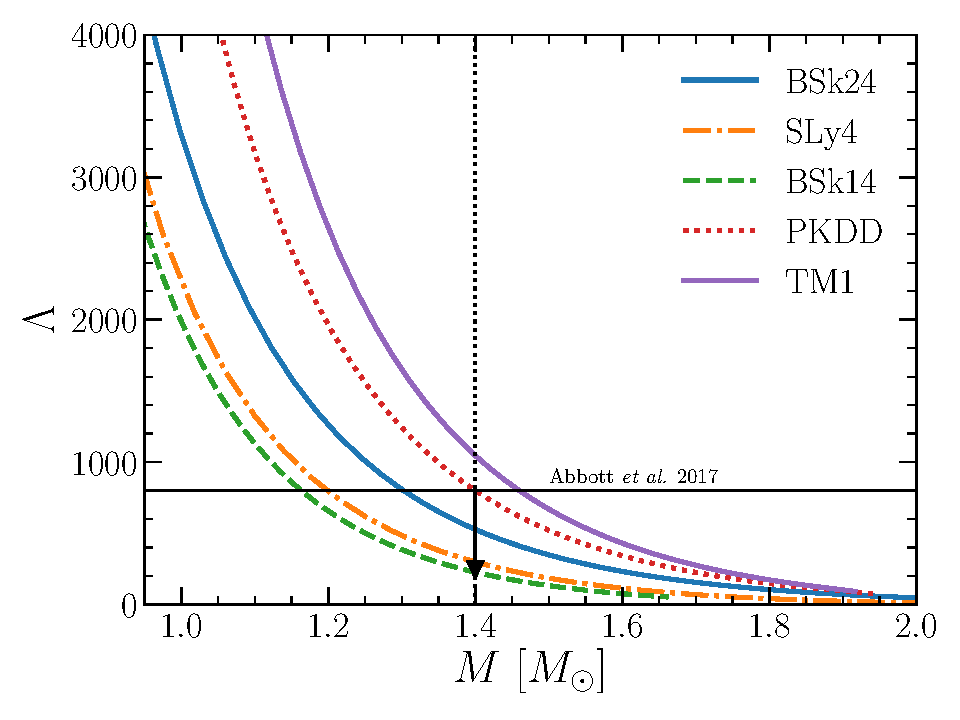
\includegraphics[width=0.9\linewidth]{figures/tidal_popular.pdf}
  \end{center}
  \caption[Tidal Love number and dimensionless tidal deformability versus 
  neutron star mass for several popular equations of state]{Tidal Love number 
    $k_2$ (upper panel) and 
    dimensionless tidal deformability $\Lambda$ (lower panel) as a function of 
    the NS mass $M$ for several popular EoS calculated within the metamodeling 
  technique. The black dotted line marks the NS canonical mass, that is
$1.4M_\odot$. In the inset of the lower panel, the value 
$\Lambda_{1.4} = 190_{-120}^{+390}$ (at $90\%$ level) inferred from GW170817 
event is represented~\cite{GW1}.}\label{fig:tidal_popular}
\end{figure}

Fig.~\ref{fig:tidal_popular} shows the variation with NS mass of $k_2$ for the 
several popular EoS that we consider in this chapter. The tidal Love number
measures how easily the bulk of the matter in a NS is deformed. In the case
of the mass being concentrated at the center of the star, the tidal deformation 
is small, and so is $k_2$. In agreement with~\cite{Hinderer2010}, we find that 
$k_2$ lies in the range $\approx 0.05-0.15$. The relative difference between
the present EoS is of the order of $\approx 35\%$ for $M=1.4M_\odot$, showing
once again the dramatic dependence on the EoS. Let us point out that the tidal 
Love number is very sensitive to the description of the crustal component of 
the EoS~\cite{Piekarewicz2019}.

The dimensionless tidal deformability is plotted as a function of $M$ in the 
lower panel of Fig.~\ref{fig:tidal_popular}. In the mass range considered, it 
is seen that the more massive the NS is, the less it gets deformed when 
orbiting another massive compact object. In the inset, we show the value of
the dimensionless tidal deformability for a $1.4M_\odot$ NS inferred from the 
GW170817 event, $\Lambda_{1.4} = 190_{-120}^{+390}$ at the $90\%$ level. We can
observe that the EoS which predict the largest tidal effects, PKDD and TM1, are 
unlikely. One can notice the tug or war between the tendency of wanting soft 
EoS, typically based on nonrelativistic Skyrme-type functionals, which predict 
small tidal deformations, and wanting very stiff EoS, typically based on 
relativistic models, to explain the glitch phenomenon as a transfer of angular
momentum from the neutron superfluid confined in the crystal lattice to the 
solid crust.

\section{Bayesian determination of the equation of state parameters}

In recent years, there has been a lot of efforts invested in the development of
the chiral effective field theory (EFT)~\cite{Drischler2016} with the aim of 
providing new constraints on the low density EoS. As we have already discussed, 
the maximum observed mass of NS~\cite{Antoniadis2013,Cromartie2020} establishes 
a stringent constraint on the EoS. Furthermore, and for the same
reason, future observations of GW signatures associated to binary NS mergers 
with LIGO and Virgo, and radius measurements from NICER will beneficial.
Bayesian inference is a statistical method which allows to account both for the 
present day knowledge on nuclear physics and NS observables for predicting the 
stellar matter EoS.

This section deals with the Bayesian determination of the EoS
parameters. The general formalism of Bayesian inference is recalled and its
application for constraining the EoS is explained in~\ref{subsec:bayes}.
In~\ref{subsec:prior}, we give the the prior distribution of EoS parameters
and a sensativity analysis of the CC transition point is carried out 
afterwards. The likelihood function, based on constraints on nuclear physics
observables, constraints on NS obervables, and physical requirements, is 
constructed in~\ref{subsec:likeli}. Finally, we present the posterior 
distribution of empirical parameters in~\ref{subsec:posterior}. A particular 
attention is paid to the correlations among parameters.

\subsection{Principle of Bayesian inference}\label{subsec:bayes}

The core of Bayesian inference is based on well-known Bayes' theorem, 
which provides an expression for the conditional probability (or posterior
probability) of $A$ given $B$,
%
\begin{equation}
  P(A|B) = \frac{P(B|A)P(A)}{P(B)}.
\end{equation}
%
In this equation, $P(B|A)$ is the conditional probability of $B$ given $A$, 
$P(A)$ is the prior probability of $A$, and $P(B)$ that of $B$.
In the model form of Bayes' theorem, one replaces $B$ by data, $A$ with 
a parameter set $\bm{X}$, and $P$ with probability density functions (PDF) 
$p$, resulting in~\cite{Bayes}
%
\begin{equation}
  p(\bm{X}|\text{data}) = \frac{p(\text{data}|\bm{X})
  p(\bm{X})}{p(\text{data})}.\label{eq:bayes1}
\end{equation}
%
The denominator is not a distribution but a normalization constant which makes 
sure that the posterior distribution $p(\bm{X}|\text{data})$ is a 
true probability distribution, by ensuring that the sum of the distribution is 
equal to 1. It is given by
%
\begin{equation}
  p(\text{data}) = \int p(\text{data}|\bm{X})p(\bm{X})
  d\bm{X}.
\end{equation}
%
The model-based formulation of Bayes' theorem, Eq.~(\ref{eq:bayes1}), is 
therefore often written as
%
\begin{equation}
  p(\bm{X}|\text{data}) \propto p(\text{data}|\bm{X})
  p(\bm{X}).
\end{equation}
%
The marginal one- and two-parameter posterior distributions can be extracted
from the posterior distribution. Then are defined respectively as
%
\begin{eqnarray}
  p(X_j|\text{data}) &=& \left\{\prod_{i \neq j} \int
  dX_i\right\}p(\bm{X}|\text{data}),\\
  p(X_j,X_k|\text{data}) &=& \left\{\prod_{i \neq j,k} 
    \int dX_i\right\}p(\bm{X}|\text{data}).
\end{eqnarray}
%

Let us describe the different components of Bayesian inference. The 
prior distribution $p(\bm{X})$ represents our knowledge or bias on the 
model parameters. It can thus be more or less informative.
$p(\text{data}|\bm{X})$ is the likelihood of observing the data given the model
parameters $\bm{X}$. It is determined from the data comparison between the 
model and the measurement via an error estimator. In that sense, the link 
between the data and the model parameters is encoded in the likelihood
distribution. 
Multiplying the prior by the likelihood function, one obtains the unnormalized 
joint posterior PDF, which corresponds to the conditional distribution of 
model parameters $\bm{X}$ given the data. Let us notice that the prior 
distribution affects the posterior distribution. 

Bayesian inference is an appealing statistical method in the sense that it 
allows to calculate the joint posterior distribution of model parameters using 
prior beliefs updated with the likelihood. In the context of NS physics, and 
from the nuclear physicist point of view, it allows for instance to update our 
knowledge on the nuclear EoS by taking into consideration the data arising from 
various astrophysical observations, that are for example the NS mass inferred
from Shapiro delay or the tidal deformability from GW measurements.
Conversely, one can account for nuclear physics constraints in the prediction 
of macroscopic observables related to NS. 
In our case, we first generate a large number of EoS, each of them being 
defined by a set of parameters $\bm{X}$, to numerically sample the prior 
parameter distribution. Then, we filter those EoS through constraints, which 
arise from physical requirements, astrophysical observations, and ab initio
calculations of SNM and PNM. This 
gives us the joint posterior distribution of model parameters, from which we 
can finally calculate the posterior EoS and make general predictions for NS 
observables. Those predictions are presented in Section~\ref{sec:general}.

Let us describe the parameter set $\bm{X}$. Our calcutation
of the stellar EoS is based on the metamodeling of nuclear matter
energy~\cite{Margueron2018a} introduced in~\ref{subsubsec:hnm}. The empirical
parameters $E_{sat}$, $n_{sat}$, $K_{sat}$, $Q_{sat}$, $Z_{sat}$, $E_{sym}$,
$L_{sym}$, $K_{sym}$, $Q_{sym}$, and $Z_{sym}$ -- which we recall are given by 
the successive derivatives of the NM energy at saturation density in isoscalar 
and isovector sectors -- therefore 
enter into the parameter set. The parameter $b$ is also added in order 
to explore different functional behaviors close to the $n\rightarrow 0$ limit.
The parameter $b$, together with the isoscalar effective mass $m_{sat}^*/m$ and 
isospin splitting $\Delta m_{sat}^*/m$, completes the parameter space, 
associated to the description of bulk matter.
In the solid crust, the metamodeling technique is supplemented by a surface 
plus curvature term in order to describe the surface properties of finite 
nuclei. Thus, one could consider adding the surface and curvature parameters, 
respectively $\sigma_0$, $b_s$, $p$, and $\sigma_{0c}$, $\beta$, as extra
parameters to $\bm{X}$. However, we have
seen in Fig.~\ref{fig:surf_fit} that the $\chi^2$ function, which evaluates the 
goodness of the fit of those parameters to experimental nuclear masses given 
BSk24 empirical parameters and $p=3$, is strongly peaked on a given set
$\bm{S}=\bm{S_{opt}}$. We expect this 
feature to be recovered for every model and we therefore choose to not include 
the surface and curvature parameters in $\bm{X}$ but to take the set 
$\bm{S_{opt}}$ that minimizes $\chi^2$, as explained in~\ref{subsubsec:cld}. 
We consider two choices for the value of the parameter $p$, which determines 
the behavior of the surface tension for extreme isospin values. Either it is 
fixed to the educated value $p=3$ or $p=\{2.5,3,3.5\}$ is considered for each
set of empirical parameters.

\subsection{Prior distribution of empirical parameters}\label{subsec:prior}

We now discuss the prior distribution of empirical parameters. We first give 
insights concerning the selected intervals for the flat prior. A senstivity 
analysis of the CC transition point is performed afterwards.

\subsubsection{Flat prior compatible with empirical constraints}\label{subsubsec:prior}

\begin{table}[!t]
  \begin{center}
    \begin{tabular}{ccccc} 
      \toprule
      \toprule
      Parameter & Unit & $N$ & Min & Max \\
      \midrule
      $E_{sat}$ & MeV & 0         & -17   & -15  \\
      $n_{sat}$ & fm$^{-3}$ & 1   & 0.15  & 0.17 \\ 
      $K_{sat}$ & MeV & 2         & 190   & 270  \\ 
      $Q_{sat}$ & MeV & 3         & -1000 & 1000 \\ 
      $Z_{sat}$ & MeV & 4         & -3000 & 3000 \\ 
      $E_{sym}$ & MeV & 0         & 26    & 38   \\
      $L_{sym}$ & MeV & 1         & 10    & 80   \\
      $K_{sym}$ & MeV & 2         & -400  & 200  \\
      $Q_{sym}$ & MeV & 3         & -2000 & 2000 \\
      $Z_{sym}$ & MeV & 4         & -5000 & 5000 \\
      $m_{sat}^*/m$ & &           & 0.6   & 0.8  \\
      $\Delta m_{sat}^*/m$ & &    & 0.0   & 0.2  \\
      $b$ & &                     & 1     & 10   \\
      \bottomrule
      \bottomrule
    \end{tabular}
  \end{center}
  \caption[Minimum value and maximum value of each of the empirical parameters
  for the prior distribution]{Minimum value and maximum value of each of the
    parameters of parameter set $\bm{X}$. The associated unit and derivative 
  order $N$ are also reported.}\label{table:prior}
\end{table}

The prior distribution of $\bm{X}$ is given by an uncorrelated ansatz and an
uniform distribution of each parameter within the interval specified in
Table~\ref{table:prior},
%
\begin{equation}
  p(\bm{X}) = \prod_{i=1}^{2(N+1)+3} \mathcal{U}(X_i^{min}, X_i^{max};X_i),
\end{equation}
%
where the parameter $X_i$ is uniformely distributed from $X_i^{min}$ to 
$X_i^{max}$. The use of a flat prior means that all possible values of 
$\bm{X}$ inside the intervals are equally likely a priori.

The range of variation for the model parameters reflect the degree of 
uncertainty on the EoS parameters, as measured by their variation in the 
functionals which reproduce succesfully low energy nuclear physics
data~\cite{Margueron2018a}. We can distinguish three groups of empirical  
parameters, depending on how well they are experimentally constrained. The 
first group consists of the low-order isoscalar parameters $E_{sat}$, 
$n_{sat}$, $K_{sat}$, the symmetry energy at saturation density $E_{sym}$, as 
well as the effective mass $m_{sat}^*$ and isospin splitting 
$\Delta m_{sat}^*/m$. These parameters are rather well determined by nuclear 
experiments, with associated relative uncertainties lower than $15\%$. The 
second group consists of the parameters that are still poorly determined by 
nuclear experiments. The uncertainties on the isoscalar skewness $Q_{sat}$, the 
slope of the symmetry energy $L_{sym}$, and the isovector incompressibility 
$K_{sym}$ are very large, yet one can expect a better accuracy to be 
reached in the near future. In particular, the determination of $L_{sym}$ is 
an highly topical issue nowadays~\cite{Li2014}. Finally, the last group 
concerns the parameters which are inaccessible by nuclear experiments to the 
present day, that is the isovector sqewness $Q_{sym}$ as well as the parameters 
of order $N=4$, $Z_{sat}$ and $Z_{sym}$ In consequence, we explore very large 
ranges for these parameters.\\
The choice of the interval for the low-density parameter, $b = [1,10]$, is 
discussed thoroughly in~\cite{Antic2019}.

\subsubsection{Sensitivity analysis of the crust-core transition
point\footnote{Partial results of the presented work have been published in 
Eur. Phys. J. A (2019) \textbf{55}: 188. With kind permission of The European
Physical Journal (EPJ).}}

Let us recall that one of the advantages of the metamodeling approach is that 
all the EoS model parameters, such as the empirical parameters, are a priori
uncorrelated. 
It is therefore possible to vary each one of them independently of the others, 
which is not feasible using specific functional behaviors such as Skyrme, 
Gogny, or the different versions of RMF, as discussed in detail
in~\cite{Margueron2018a,Margueron2019}. 
Indeed, common functionals describing infinite NM have a smaller number of 
parameters compared to the metamodel, which creates a priori correlations that 
are not fully controlled. If we take the example of Skyrme forces, the density 
dependence of SNM is controlled by only three parameters, which are fixed 
to reproduce the coordinates of the saturation point: $n_{sat}$, $E_{sat}$, and 
$K_{sat}$. Thus, the isoscalar skewness $Q_{sat}$ is correlated with the 
three other parameters, and it turns out that this correlation is not the same, 
for instance, in Skyrme, Gogny, or in RMF functionals~\cite{Margueron2019}. A 
similar argument applies to the symmetry energy: when the density dependence of 
the symmetry energy is governed by a single parameter as assumed in heavy ion 
transport models, an isosoft behavior at suprasaturation density is necessarily 
associated to an isostiff behavior at subsaturation density, while more 
complicated behaviors are possible~\cite{Margueron2019}. The independent 
variation of the different empirical parameters allows a simple determination 
of the most influential parameters impacting a given observable under study. 

\begin{figure}[!t]
\begin{center}
  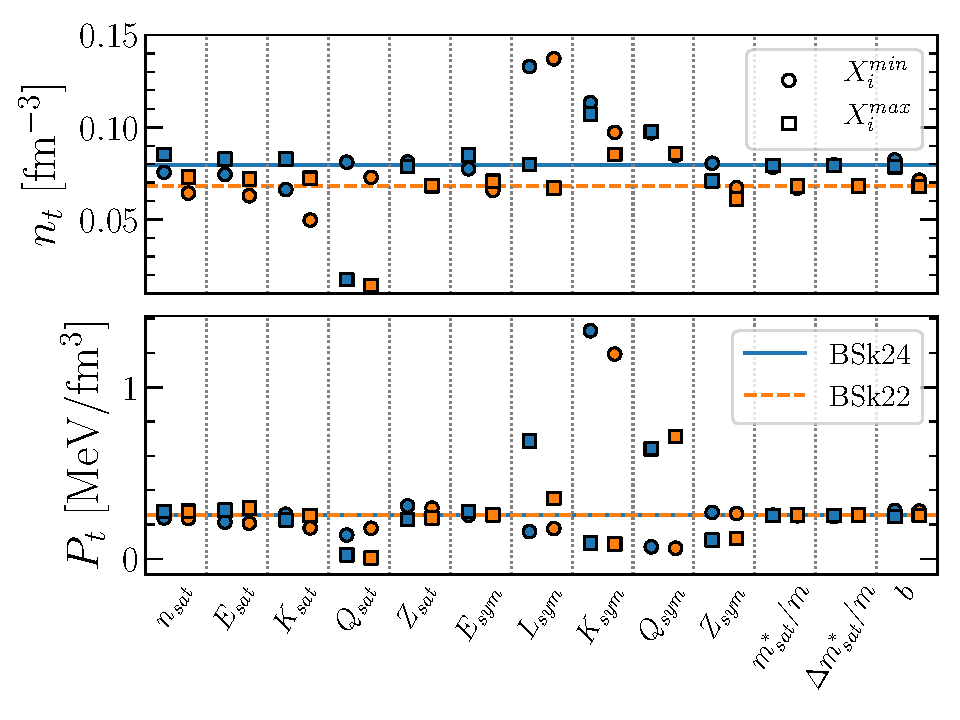
\includegraphics[width=0.9\linewidth]{figures/sensana.pdf}
\end{center}
\caption[Sensitivity analysis of the crust-core transition point for
BSk24 and BSk22]{Sensitivity analysis of the transition density $n_t$ (upper 
panel) and transition pressure $P_t$ (lower panel) with respect to EoS 
parameters. $p=3$ is fixed and two different reference point are chosen:
BSk24 parameters (solid blue lines) and BSk22 parameters (orange 
dashed lines). For each parameter, the symbols on left (blue) correspond to 
BSk24 and those on right (orange) to BSk22. Circles and squares are
respectively associated to the minimum value $X_i^{min}$ and maximum value
$X_i^{max}$ of the parameter, which are listed in 
Table~\ref{table:prior}.}\label{fig:sensana}
\end{figure}
 
Such a sensitivity analysis is presented in Fig.~\ref{fig:sensana} for the 
CC transition density $n_t$ and transition pressure $P_t$. The reference 
metamodel used in the sensitivity analysis can have an influence. For this 
reason, the sensitivity analysis varying one by one the EoS parameters is 
performed around two different reference parameter sets $\bm{X_{ref}}$, namely 
the parameter set corresponding to the BSk24 functional (solid blue lines), and 
the one corresponding to the BSk22 functional (dashed orange lines). For both 
of them, we fix $p=3$ as well as $b=10\ln(2)$.

The range of variation for each of the EoS parameters 
correspond to the intervals for the prior distribution $p(\bm{X})$ specified in 
Table~\ref{table:prior}. Let us however notice that some sets produce nonviable 
EoS, for which a solution for the CC transition point cannot be found. This
occurs in particular when varying the value of the isovector incompressiblity 
parameter $K_{sym}$ with BSk24 as reference parameter set. Indeed, we find 
an extremely soft behavior for the symmetry energy for the minimum value 
$K_{sym}^{min}=-400$ MeV. In that very situation, we increase the minimum value 
of the parameter to $K_{sym}^{min} \approx -300$ MeV so as to find a solution 
for $n_t$ and $P_t$.

The symbols in Fig.~\ref{fig:sensana} give the transition density and 
pressure domain obtained when the EoS parameters are one by one varied around 
the reference model, within the interval of Table~\ref{table:prior}. More
specifically, circles and squares are respectively associated to the minimum
value and maximum value of each parameter.
Since the uncertainty on the different parameters is not the same, the 
relative distance between circles and squares is a qualitative measurement of 
the propagation of the uncertainty on the transition point brought by each 
parameter. We can see that the sensitivity of each parameter depends on the 
value of the other parameters, that is on the chosen reference set 
$\bm{X_{ref}}$. Still, universal trends clearly emerge. We can see that the CC 
phase transition, at variance with the 
standard liquid-gas of SNM, is virtually insensitive to isoscalar parameters. 
Even if extremely large variations of $Q_{sat}$ and $Z_{sat}$ are considered, 
see Table~\ref{table:prior}, the influence of the isoscalar parameters in the 
transition pressure is almost negligible, and it is a bit larger for $n_t$ but 
still smaller than the isovector parameters. This underlines the importance of 
the energetics of the neutron gas on the transition point. Concerning the 
isovector sector, we can see that $L_{sym}$ is the most important 
parameter as far as the transition density is concerned. This result is in 
agreement with previous findings by many authors~\cite{Ducoin2011} and was
already anticipated in~\ref{subsec:ccfromc}.
The symmetry energy at saturation $E_{sym}$ and the effective mass splitting
$\Delta m_{sat}^*/m$ do not play any role on the transition, which can be 
partially explained by the fact that these parameters are already relatively 
well constrained. The transition density and pressure show also a great 
sensitivity to the isovector incompressibility parameter $K_{sym}$. 
This can explain why the transition pressure exhibits an irregular behavior 
when plotted as a function of $L_{sym}$ (see Fig.~\ref{fig:cctp_lsym}): the 
different functionals considered in the literature have very different values 
of $K_{sym}$, which blurs the correlation with $L_{sym}$. This effect is also 
amplified by the fact that, depending on the reference point, the dependence of 
$P_t$ with $L_{sym}$ is not monotonic. Finally, we can notice that the 
influence of the fully unknown high order derivatives $Q_{sym}$ and $Z_{sym}$, 
though less important than the one of $L_{sym}$, is not negligible and 
comparable to the one of the isovector surface energy parameter $p$ that can be 
inferred from Fig.~\ref{fig:cctp_lsym}. We have checked that similar 
conclusions can be drawn if the sensitivity analysis is performed using the 
definition of the transition point from the dynamical 
spinodal~\cite{Antic2019}.

\subsection{Determination of the likelihood function}\label{subsec:likeli}

The likelihood function corresponds to the probability of observing the data
given the model parameters $\bm{X}$. In the context of our analysis, it is
defined as
%
\begin{equation}
  p(\text{data}|\bm{X}) = w_{LD}(\bm{X}) \times 
  w_{HD}(\bm{X}) \times p_{\text{AME2016}}(\bm{X}).
\end{equation}
%
In this expression, $w_{LD}$ and $w_{HD}$ are strict filters that concentrate
on constraining the low density EoS and high density EoS, respectively. Both 
filters are given by sharp $\delta$ functions that output $1$ if the constraint 
is satisfied, and $0$ otherwise. 
Constraints on nuclear physics observables, yielding the filter $w_{LD}$ and 
the probability $p_{\text{AME2016}}$ are presented in~\ref{subsubsec:ldconst}.
In~\ref{subsubsec:hdconst}, we present the
constraints corresponding to the filter $w_{HD}$, which are associated to 
general physical requirements and measurements of NS observables. 

\subsubsection{Constraints on nuclear physics
observables}\label{subsubsec:ldconst}

Let us concentrate first on the strict filter $w_{LD}$, herafter referred to as
low density (LD) filter. It is introduced to verify whether the metamodel 
associated to a set of parameter $\bm{X}$ is compatible with the recent chiral
effective field theory (EFT) calculations for SNM and PNM by Drischler 
\textit{et al.}~\cite{Drischler2016}. The authors have calculated the energy
per particle for several values of isospin at low density within the many-body
perturbation theory, based on a set of seven different Hamiltonians with chiral 
NN and three-nucleon interactions.

\begin{figure}[!t]
\begin{center}
  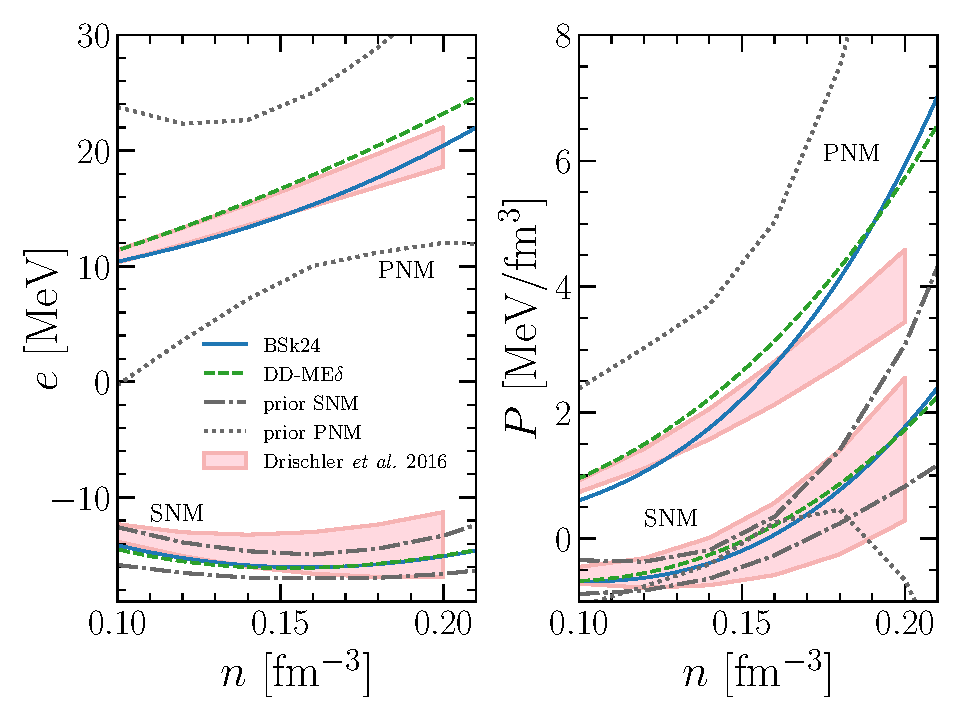
\includegraphics[width=0.9\linewidth]{figures/drischler.pdf}
\end{center}
\caption[Energy per nucleon and pressure of nuclear matter versus density from 
chiral effective field theory caclulations]{Energy per nucleon 
  (left panel) and pressure (right panel) as a function of density for both SNM 
  and PNM from chiral ETF calculations of~\cite{Drischler2016} (pink
bands). The predictions of BSk24 and DD-ME$\delta$ functionals are represented 
in solid blue lines and dashed green lines, respectively. The gray lines
give the minimum and maximum values of the prior 
distribution.}\label{fig:drischler}
\end{figure}

The resulting predicted bands for energy per nucleon as well as pressure of SNM
and PNM are shown in Fig.~\ref{fig:drischler} (pink pands), together with 
the predictions of the popular BSk24 (solid blue lines) and DD-ME$\delta$ 
(green dashed lines) functionals. 
The pressure band is calculated by taking the density derivative of the energy 
per nucleon for the seven Hamiltonians, thus only few density dependencies of 
the pressure are explored. This can explain why even realistic models such as 
BSk24 are not compatible with the theoretical band for the 
pressure of PNM above $\approx n_{sat}$. It is therefore debatable whether 
we should add the chiral EFT bands for pressure of NM in our list of
constraints defining our pass-band filters $w_{LD}$. In the following, we will 
not consider this particular contraint by default, yet we will still 
investigate how it affects the posterior distribution EoS in~\ref{sec:general}.
In the context of the pass-band filter $w_{LD}$, the chiral ETF predicted 
bands are widened by $5\%$ in order to account for other existing ab initio 
calculations in an effective manner. In addition, we will not apply the filter
in the low density region $n < 0.10$ fm$^{-3}$ because the width of the band 
becomes extremely small, causing numerical issues.

The minimum values and maximum values of the prior distribution are also
represented in Fig.~\ref{fig:drischler} (gray lines). Let us notice that one 
can the infer the posterior band graphically by the comparison with the chiral 
ETF bands. Interestingly, the graphically inferred posterior band of the 
prior energy per nucleon and pressure of SNM around saturation density is 
narrower than the one corresponding to the ab initio calculation. The reason is
that low energy nuclear physics experiments provide strong empirical
constraints for SNM~\cite{Margueron2018a}, which have been embedded 
effectively in the intervals for the empirical parameters of the prior
distribution in Table~\ref{table:prior}. The same is not true for the PNM case. 
Indeed, the present day knowledge on the empirical parameters of the 
isovector sector is insufficent. For this reason, we can see that the 
corresponding ab initio bands are very thin in comparison to the prior 
distribution.

% pame2016
We now turn the calculation of the probability $p_{\text{AME2016}}$, which 
describe the ability of the CLDM defined from a parameter set $\bm{X}$, to fit 
the measured nuclear masses of the AME2016~\cite{Huang2017}. The goodness of 
fit is evaluated by the reduced $\chi^2$, Eq.~\ref{eq:chi2}. We can define the 
associated likelihood probability as
%
\begin{equation}
  p_{\text{AME2016}}(\bm{X}) = \exp\left[-\frac{1}{2}\chi_\nu^2(\bm{X})\right].
\end{equation}
%
 
\subsubsection{Physical requirements and constraints on neutron star 
observables}\label{subsubsec:hdconst}

The filter $w_{HD}$, hereafter referred to as high density (HD) filter, is
applied subsequently to the LD filter $w_{LD}$. It imposes general physical 
constraints to the global density behavior of the functional, as follows:
%
\begin{itemize}
  \item the positiveness of the symmetry energy at all densities,
  \item the stability of the EoS,
  \item the causality condition, $0 < c_s/c < 1$,
  \item the maximum observed NS mass, $M_{max}(\bm{X}) \geq M_{max}^{obs}$,
\end{itemize}
%
where $M_{max}(\bm{X})$ is the maximum mass supported by the EoS calculated for 
a parameter set $\bm{X}$, and $M_{max}^{obs}$ is the maximum observed NS mass. 
By default we choose $M_{max}^{obs} = 1.97M_\odot$, which corresponds to 
a $1\sigma$ conservative estimate, based on the observation of PSR 
J0348+0432~\cite{Antoniadis2013}. 
Let us however notice that it does not correspond to the mass of the heaviest 
NS observed to the present day~\cite{Cromartie2020}. The reason is that the
observation of PSR J0740+6620 with $M = 2.14_{-0.09}^{+0.10}M_\odot$ is very 
recent and it was not yet published at the time of this study.

As we have already discussed, for a given functional, the redefinition of 
high-order parameters $Q_{sat}$, $Z_{sat}$, $Q_{sym}$, and $Z_{sym}$ is 
necessary in order to achieve faster convergence at high density and thus 
to recover the right value for the maximum mass. 
The LD filter is applied in the density range $0.10$ fm$^{-3}$ $< n < 0.20$ 
fm$^{-3}$, that is in the vicinity of the saturation density $n_{sat}$. 
In this density range, the effect of parameters of orders $N \geq 2$ on the 
energy per nucleon of NM is very small, and consequently we can legitimately 
expect that $Q_{sat}$, $Z_{sat}$, $Q_{sym}$, and $Z_{sym}$ will not be strongly
constrained by the LD filter. In that sense, for each parameter set passing 
through the pass-band filter $w_{LD}$, we sample $10$ new parameter sets by 
randomly drawing new values for the high-order parameters with the aim of 
obtaining more sets passing through both LD and HD filters.
Nevertheless, we have seen in Fig.~\ref{fig:sly4_nt} that the inclusion of
orders $N \geq 2$ is important to precisely estimate the CC transition point.
In that sense, $n_t$ and $P_t$ will be calculated using the high-order 
parameters that originate from the passage through the LD filter and which are 
kept by the HD filter.

The possibility of a negative symmetry energy at high density was sometimes 
evocated in the literature~\cite{Li2017,Wiringa1988}. 
However, extremely soft functionals are generally incompatible with the maximum 
mass constraint, thus relaxing the condition of the positiveness of the 
symmetry energy will not alter our results.

Finally, let us notice that we do not include the constraint on the tidal
deformability inferred from the GW170817 event~\cite{GWtidal} in the $w_{HD}$ 
filter, the reason being that we are interested in confronting our results with 
the observations of LIGO and Virgo.

\subsection{Posterior distribution of empirical
parameters}\label{subsec:posterior}

% discuss the importance of filters?

\section{General predictions for neutron star observables}\label{sec:general}

% should i add a subsection 'Posterior distribution of NS observables'?

\subsection{Confrontation with GW170817 event} % 1

% general presentation of the gw170817 event
% say that we identify it to a bns because we observed em counterparts
%   -> multimessenger era

\subsubsection{Equation of state} % 1

\subsubsection{Mass-radius relation} % 1.5

% speed of sound expansion allows for phase transition, unlike the mm
% -> lower radius found in 1908.10352 could be the sign of a pt to quarks?

\subsubsection{Tidal deformability} % 2

% mchirp is measured very precisely
% was measured for the first time for gw170817 event allowing to calculate the
%   m1-m2, lambda1-lambda2 relations

\subsection{Bayesian analysis of the crust-core transition} % 4

% surface figures (prior/posterior)
% corr(Pt,Ksym) (link with chapter 1)
% correlation with isovector bulk parameters is softened if one consider p as a
%   free parameters (see corr matrix)

\subsection{Crustal moment of inertia and pulsar
glitches}\label{subsec:gli_stats} % 4

% explain pulsar glitches phenomena
% give the hypothesis explaining the phenomena
% superfluid neutrons in the crust
% is the crust enough? -> bayesian approach to consider every models (not only
%   relativistic or skyrme functionals as two separate families)
% the crust moment of inertia is calculated following eq given in 2.1.2. the
%   calculation is stopped at the crust-core interface
% report results

\section{Conclusion} % 1

% word on machine learning
% one can expect more constraints in the future with nicer and lvc
